\chapter{Metodo proposto}
\label{metodo}


In questo capitolo si discuterà del workflow seguito per ottenere i risultati che saranno esposti nel Capitolo \ref{risultati}. L'implementazione degli aspetti esposti è stata realizzata in Python, con la libreria PyTorch. 

\section{Feature Extractor: DINOv2}
Come anticipato, utilizziamo DINOv2 come feature extractor per la nostra sperimentazione. Il modello di DINOv2 pre-allenato è stato scaricato dalla pagina GitHub di Meta \cite{dinov2_github}. Si tratta sempre di ViT/14, con dimensione dei patches di \(14 \times 14\) pixels (per maggiori informazioni Appendice \ref{vit}). 

Dopo che il modello di DINOv2 viene allenato nelle modalità descritte nella Sezione \ref{dinov2}, si eliminano il Teacher, il mascheramento e le teste di proiezione. Di fatto, quindi, stiamo prendendo i pesi del ViT già allenati e congelati e usandoli per estrarre delle rappresentazioni delle nostre immagini.


\section{Features}
Per la classificazione utilizziamo due diverse tipologie di features estratte da DINOv2: il token [CLS] e l'AVG patch.

\begin{figure}[t]
    \centering
    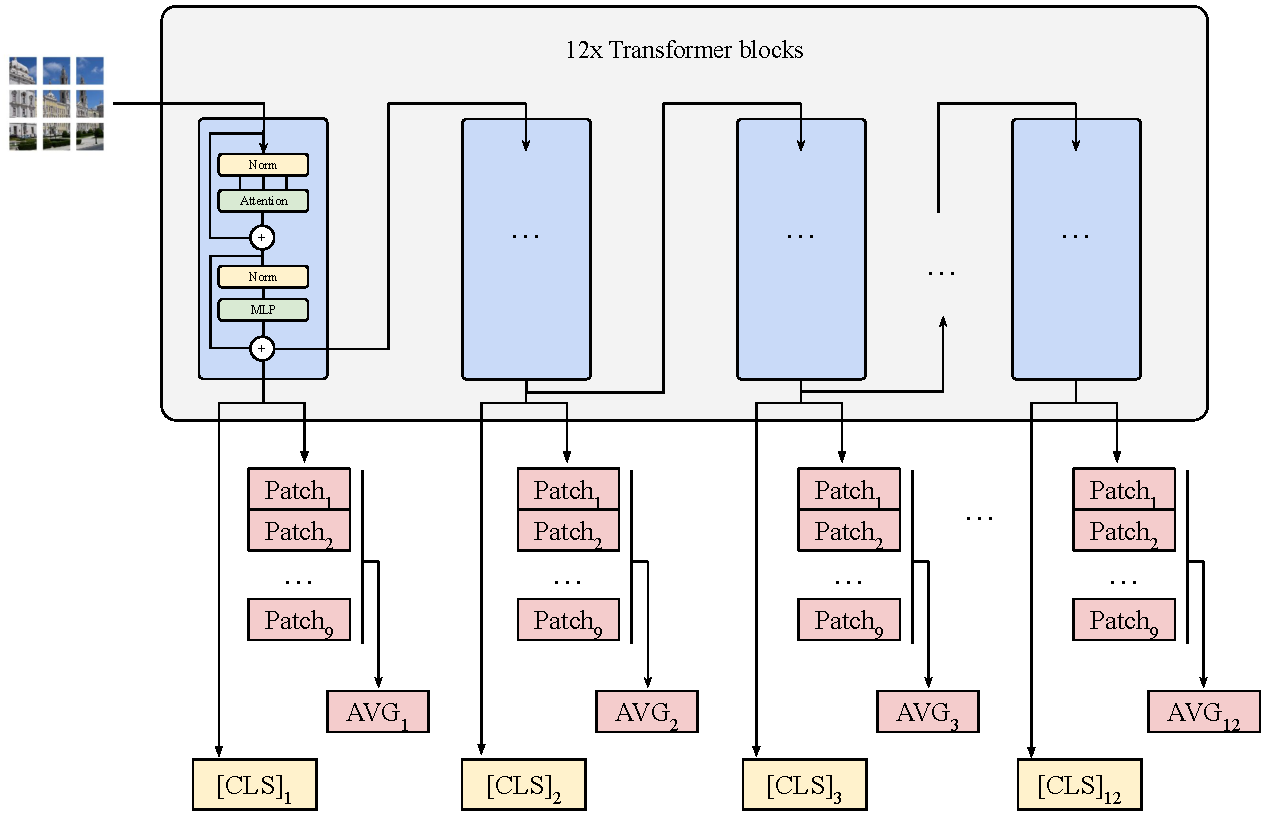
\includegraphics[height=10cm]{Immagini/metodo/tokens_arch.pdf}
    \caption{Estrazione dei token CLS e patch AVG dal ViT di DINOv2}
    \label{fig:token}
\end{figure}

\begin{figure}[t]
    \centering
    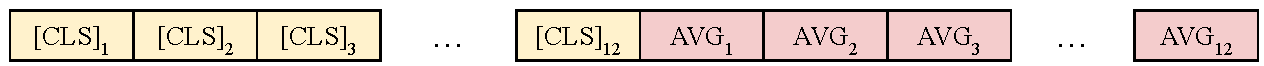
\includegraphics[width=\textwidth]{Immagini/metodo/tokens_conc.pdf}
    \caption{Concatenazione delle features}
    \label{fig:token_conc}
\end{figure}

\subsection{CLS}
Come meglio descritto nell'Appendice \ref{cls}, CLS è un token interamente appreso durante l'allenamento di DINOv2, e quindi del ViT sottostante, che raccoglie il contenuto informativo di tutta l'immagine. Per questo motivo, è generalmente utilizzato come feature principale in task di classificazione, specialmente semantica.

\subsection{AVG patch}
Il ViT produce un vettore di rappresentazioni per ciascuno dei patch in cui è suddiviso nell'immagine. Generalmente questi vengono ignorati, [CLS] è il vettore di embeddings che viene utilizzato nella classificazione (Figura \ref{fig:arch_vit}). 

Nonostante ciò, sia nel paper che ha introdotto i Vision Transformers \cite{vit} che in quello di DINOv1 \cite{dino} si sperimenta anche utilizzando come vettore di features la media elemento per elemento delle rappresentazioni dei patches. Questo è uno degli approcci usati prima dell'introduzione di [CLS] da parte di BERT. Si dimostra che con determinati learning rates, questo vettore produce nei ViT risultati che si avvicinano a quelli di CLS.

Per questo motivo utilizziamo anche questo vettore media come feature su cui sperimentare, concatenandolo sequenzialmente al vettore estratto da [CLS].

\subsection{Combinare le features di più layers}
Un'ulteriore sperimentazione che già nella prima versione di DINO viene fatta è quella di non utilizzare solamente l'output preso dal token [CLS] all'ultimo layer, ma di concatenare gli outputs provenienti dai diversi \textit{transformer blocks} precedenti all'ultimo, che compongono il ViT (Figura \ref{fig:token}). Si osserva che questo può portare ad un miglioramento delle prestazioni del modello. L'intuizione è che i layer precedenti all'ultimo possano raccogliere informazioni a diversi livelli di astrazione, come succede nelle CNN.

Adottiamo questa tecnica sia per il token [CLS] che per l'AVG patch. Supponendo di scegliere un numero \(l\) di layers da cui estrarre [CLS] e un numero \(m\) di layers su cui fare la media dei patch, il vettore di features finale sarà la concatenazione degli \(l\) vettori CLS, seguito dalla concatenazione degli \(m\) vettori media (Figura \ref{fig:token_conc}).

\vspace{3mm}
\section{Classificatore}
Usiamo i due datasets descritti nel prossimo capitolo per allenare separatamente il nostro classificatore, con diverse combinazioni delle features proposte. Estraiamo in anticipo tutte le features per tutte le immagini appartenenti a ciascun dataset dal modello di ViT scelto (ViT-S, ViT-B, ViT-L) e le salviamo in un file \textit{.pt}. In questo modo possiamo lanciare più scripts di evaluation senza dover ricalcolare per ciascuno i vettori di rappresentazione per ogni immagine.

Come classificatore proviamo un semplice layer lineare, pratica standard nei protocolli di valutazione dei modelli:
\begin{equation}
    y = Wx + b
\end{equation}
dove \(x\) il vettore di features scelte, \(W\) è la matrice dei pesi del layer e \(b\) il bias, entrambi appresi.

Proviamo poi anche un MLP con 1 hidden layer e funzione di attivazione ReLU:
\begin{equation}
    y = W_2 \sigma(W_1x+b_1)+b_2
\end{equation}
Aggiungiamo anche un dropout per mitigare il problema dell'overfitting, più probabile in un MLP che in un layer lineare. La dimensione del layer nascosto è pari alla metà di quella del layer in input.

In entrambi i casi, il vettore di features in input viene mappato su un vettore in output di dimensione pari al numero di classi presenti in ciascun dataset (9 e 17).

\section{Loss}
La loss utilizzata è la binary cross-entropy (BCE) with logits. Se \(x\) è uno dei logits prodotti in output dall'ultimo layer e \(y\) l'etichetta reale corrispondente a quella immagine per quella classe (0/1), allora
\begin{equation}
    \text{BCEwithLogits}(x, y) = BCE(\sigma(x), y)
\end{equation}
dove:
\begin{itemize}
    \item \(\sigma(x)\) è la funzione sigmoide applicata al logit, che lo porta nel range \([0, 1]\), rendendolo interpretabile come una probabilità:
    \begin{equation}
        p  = \sigma(x) = \frac{1}{1 + e^{-x}}
    \end{equation}
    \item La binary cross-entropy è calcolata come:
    \begin{equation}
        BCE(p, y) = -(y\log(p) + (1-y)\log(1-p))
    \end{equation}
\end{itemize}
La funzione BCE tratta ogni classe come una classificazione binaria (0 o 1), separatamente dalle altre. Per questo motivo può essere preferibile nella classificazione multi-label e non richiede che le immagini siano passate alla rete più di una volta. Per lo stesso motivo, viene utilizzata sigmoide al posto di softmax: mentre softmax normalizza un intero vettore di predizioni, \(\sigma\) lavora su ciascun logit separatamente, rendendola adatta in contesto di classificazione binaria.


\section{Preparazione delle immagini}
Per ridurre il numero di patches all'interno di una immagine, e quindi il tempo e lo spazio in memoria richiesto per estrarne le features, è necessario ridimensionare tutte le immagini date in input a DINOv2. Scegliamo di porre il lato più lungo di ciascuna di esse a dimensione 500 e di scalare la seconda dimensione di conseguenza. Inoltre, le dimensioni devono essere multiple di 14, in modo che si possano produrre un numero intero di patch 14x14. Per questo motivo, facciamo un crop centrale dell'immagine ridimensionata in modo che i suoi lati risultino multipli di 14.

Per velocizzare ancora di più il processo di estrazione delle features, sarebbe opportuno che le immagini siano quadrate, in modo da poterle mandare in batch alla rete. Questo, però, potrebbe risultare problematico nel contesto della composizione fotografica. Produrre delle immagini quadrate a partire da fotografie rettangolari richiede di fare crop, che inevitabilmente cambia la posizione relativa dei soggetti all'interno della composizione, distruggendo la regola dei terzi. Alternativamente, potremmo pensare di fare uno stretching dell'immagine fino a proporzioni quadrate, ma questo rischia di distorcere le leading lines, soprattutto quelle curve. Si decide quindi di mantenere gli aspect ratio originali, a scapito delle prestazioni.